\chapter{Normalisierung}
\section{Rasterisierung}

\begin{wrapfigure}{R}{0.4\textwidth}
  \vspace{-20pt}
  \begin{center}
    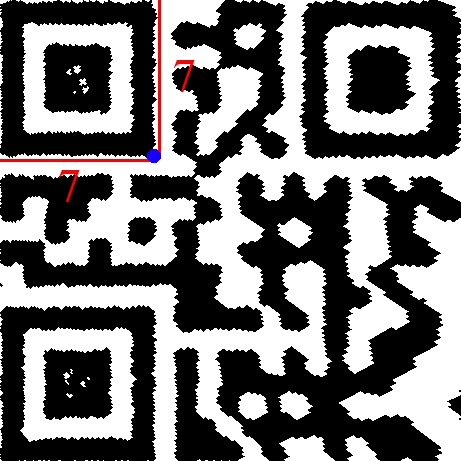
\includegraphics[scale=0.25]{images/Gitter_step.png}
  \end{center}
  \vspace{-10pt}
  \label{fig:raster-qrcode}\caption{Rasterlänge berechnen}
  \vspace{-10pt}
\end{wrapfigure}

Nach der perspektivischen Transformation, liegt das extrahierte Bild in einem $n\times n$ großem binarisiertem Zustand vor. Nun muss der \QRCode rasterisiert werden.

Man betrachte dazu die untere rechte Ecke des \olfpn. Es ist bekannt, dass ein \fp die Dimension $7 \times 7$ hat, sodass man die $x$ bzw. $y$-Koordinate der genannten Ecke durch $7$ dividiert. Dies liefert die Zellenlänge $z$ des Rasters, woraus sich die Anzahl der Module $m$ via Division von $n$ mit $z$ berechnen lässt. Im Normalfall gilt jedoch $m \notin \mathbb{Z}$.
Es ist jedoch bekannt, dass ein \QRCode nur 
\begin {equation*}
	17 + 4 \cdot version
\end{equation*}
für $version \in \left\{1, ..., 40\right\} \subset \mathbb{N}$, Module besitzen kann.
\begin{figure}[h]
\centering
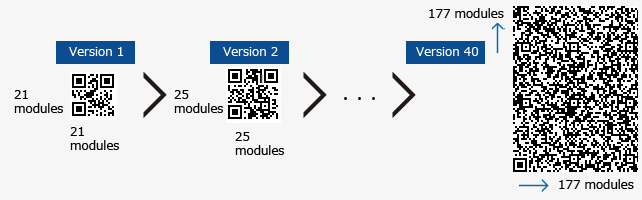
\includegraphics[scale=0.5]{images/QRVersion.png}
\label{fig:version-qrcode}
\caption{Mögliche Modulgrößen von \QRCodes}
%\footnote{Quelle:\url{http://www.qrcode.com/en/img/version/versionVarietyImage.png}}
\end{figure}

\noindent Die Anzahl der geschätzten Module $m$ wird zur Berechnung der nächsten ganzzahligen Versionsnummer genutzt:
\begin{equation*}
	version = round((m-17)/4)
\end{equation*}
Die zur Versionsnummer gehörenden Anzahl der Module ist dann gegeben durch:
\begin{equation*}
	modules = 17+4 \cdot version
\end{equation*} 
Die Zellenlänge des Rasters berechnet sich letztendlich aus Divison von $n$ mit $modules$. Diese Zellenlänge wird für den folgenden Schritt der Normalisierung benötigt.

\section{Normalisierung}
Die Normalisierung wird mithilfe des Rasters durchgeführt, indem \emph{majority votes} pro Zelle den Pixelwert des normalisierten \QRCodes festlegen.
Das Ergebnis ist ein $modules \times modules$ großer normalisierter \QRCode.

\begin{figure}[h]
\centering
\begin{subfigure}[t]{0.45\textwidth}
\centering
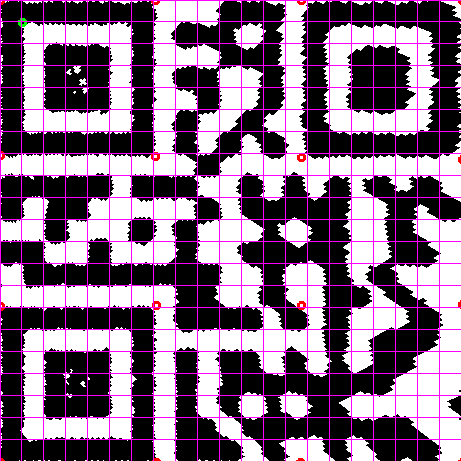
\includegraphics[scale=0.25]{images/gitter.png}
\caption{Extrahiert mit Raster}
\label{fig:version-qrcode}
\end{subfigure}
\begin{subfigure}[t]{0.45\textwidth}
\centering

\includegraphics[scale=5.5]{images/qrcode-adler.png}
\caption{Normalisierter \QRCode}
\label{fig:final}
\end{subfigure}
\caption{Normalisierung des \QRCodes.}
\end{figure}

\section{Verifikation}
Um fälschlicherweise erkannte \QRCodes zu vermeiden, wird im Anschluss eine Verifikation durchgeführt. Dies geschieht, indem die Pixel des normalisierten Bildes, wo die Finder Patterns und Timing Patterns liegen, mit denen eines Standard \QRCodes der entsprechenden Version verglichen werden.
\begin{figure}[h]
\centering
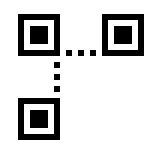
\includegraphics[scale=0.5]{images/verifikation.png}
\label{fig:version-qrcode}\caption{Finder und Timing Patterns eines Standard \QRCodes der Version $1$}
\end{figure}
\\
Ist die Übereinstimmung des normalisierten Bildes mit einem Standard \QRCode geringer als $85\%$, so wird, falls möglich, die Normalisierung und die Verifikation mit einer Versionsnummer von $\pm 1$ wiederholt. Dadurch wird Rundungsfehlern bei der Rasterisierung vorgebeugt. Sind alle Übereinstimmungen unter $65\%$, so wird der \QRCode verworfen, andernfalls wird der \QRCode mit der höchsten Übereinstimmung gewählt und gespeichert.

Für den Fall, dass mehr als ein valider \QRCode gefunden wurde, wird am Ende, im Rahmen der Aufgabenstellung, der \QRCode mit der höchsten Übereinstimmung ausgegeben.